\documentclass{tufte-handout}

\usepackage{librecaslon}
\usepackage{fancyhdr}
\usepackage{hyperref}
\usepackage{tcolorbox} % needed for the text boxes
\usepackage{xcolor}
\usepackage{setspace}
\usepackage{graphics}
\usepackage{./tuftefoot}

% Set header and footer
\pagestyle{fancy}
\fancyhf{}
\lfoot{\includegraphics[height=1cm,keepaspectratio]{../img/i2i}}
\cfoot{\includegraphics[height=1cm,keepaspectratio]{../img/wb}}
\rfoot{\includegraphics[height=1cm,keepaspectratio]{../img/analytics}}

% Put checkbox to the left of the text
\def\LayoutCheckField#1#2{% label, field
	#2 #1%
}

% Line spacing
\onehalfspacing

% Define DIME Analytics visual identity colors
\definecolor{fontcolor}{HTML}{7A0569}

\titleformat{\section}%
{\Large\rmfamily\bf\color{fontcolor}}% format applied to label+text
{\llap{\colorbox{fontcolor}{\parbox{1.5cm}{\hfill\huge\color{fontcolor}\thesection}}}}% label
{2pt}% horizontal separation between label and title body
{}% before the title body
[]% after the title body

\titleformat{\subsection}%
{\large\rmfamily\color{fontcolor}}% format applied to label+text
{}% label
{1.5pt}% horizontal separation between label and title body
{}% before the title body
[]% after the title body

\newcommand{\dimeCheckBox}[1]{\CheckBox[height=0.01cm, width=0.4cm, bordercolor=gray]{#1}}
\newcommand{\dimeTextField}[3]{\TextField[name=#1, height=0.3cm, width=#2, bordercolor=gray]{#3}}


\newcommand{\titleBox}[1]{
	\begin{tcolorbox}
		[colframe = fontcolor,
		colback = fontcolor,
		sharp corners,
		halign = flush center,
		valign = center,
		height = 0.3\textwidth,
		after skip = 1cm]
		#1
	\end{tcolorbox}
}


% ------------------------------ End of preamble ---------------------------------------------
\begin{document}
	\begin{fullwidth}

\titleBox{
	\textcolor{white}{\LARGE{\textbf{DIME Analytics \\ Reproducibility Package Checklist}} \\
	\Large\textbf{{v1.4}}}
}

	\section*{Required Content and Practices}

	The reproducibility package must be shared as a .zip file, GitHub link or shared folder containing the items listed below.
	
	\subsection{1. \, Files}
	
	\begin{itemize}
		\setlength\itemsep{-0.1em}
		\item[] \dimeCheckBox{A filled version of this checklist.}
		\item[] \dimeCheckBox{A README file describing the folders and datasets included in the package, and any general or ad-hoc instructions about the directory structure or for the code to run.}
		\item[] \dimeCheckBox{A PDF version of the research output being reviewed (paper, brief, report).}
	\end{itemize}

	\subsection{2. \, Code}

	\begin{itemize}
		\setlength\itemsep{-0.1em}
		\item[] \dimeTextField{software}{8cm}{Software used (including version):}
		\item[] \dimeTextField{os}{8cm}{Operating system used:}
		\item[] \dimeCheckBox{All scripts needed to reproduce the analysis is included in the reproducibility package.}
		\item[] \dimeCheckBox{The reproducibility package includes a \textbf{master script}.}
		\item[] \dimeTextField{master}{11cm}{Master script path and name:}
	\end{itemize}

	\vspace{.6em}
	\noindent The items below only apply if the reproducibility package includes a master script.

	\begin{itemize}
		\setlength\itemsep{-0.1em}
		
		\item[] \dimeTextField{time}{2.5cm}{\textbf{Approximate time} it takes to recreate all results from the the master script: }
		\item[] \dimeTextField{ram}{2.5cm}{RAM size of computer used to calculate time:}

		\item[] \dimeCheckBox{The master script re-creates all raw outputs (e.g. tables and figures) when executed.}

		\item[] \dimeCheckBox{All raw outputs are re-created \textbf{as they appear in the paper}, requiring no manual changes.}

		\item[] \dimeCheckBox{All raw outputs are re-created in the same folder structure as they were submitted in the reproducibility package.}

		\item[] \dimeCheckBox{The master script \textbf{installs any commands required} (e.g. from SSC in Stata, CRAN in R, etc.).}

		\item[] \dimeCheckBox{In Stata, the master do file sets \textbf{critical configurations} such as \texttt{version}, \texttt{matsize}, and \texttt{varabbrev} (either sets directly or through a wrapper command such as \texttt{ieboilstart} from \texttt{ietoolkit}).}

		\item[] \dimeCheckBox{In R, all necessary packages to run the code are loaded in the master script.}
		\item[] \dimeCheckBox{All file paths in the code use only forward slashes, i.e. \texttt{C:/users/...}.}

		\vspace{0.3em}
		\item[] Select only one of the following two options.
		\vspace{-0.3em}
		\begin{itemize}
			\setlength\itemsep{-0.1em}
			\item[] \dimeCheckBox{Results are reproducible using the \textbf{most recent version} of the user-written commands (as available in CRAN/SSC) at the time of submitting the reproducibility package.}

			\item[] \dimeCheckBox{The master script installs the \textbf{exact version} of each package required, either from within the reproducibility package itself, or from a remote location.}
		\end{itemize}
	\end{itemize}

	\subsection{3. \, Data}

	The reproducibility package includes:
	\begin{itemize}
		\setlength\itemsep{-0.1em}
		\item[] \dimeCheckBox{Fully de-identified data. \textbf{Any exception where DIME Analytics needs to access restricted or sensitive data sets will require additional ethics and security measures, and will be handled on a case-by-case basis.}}

		\item[] \dimeCheckBox{All data necessary to run the master script that reproduces the analysis.}
	\end{itemize}

	\noindent Indicate the stage of the data this package begins reproducibility from (select only one):
	\begin{itemize}
		\setlength\itemsep{-0.1em}
		\item[] \dimeCheckBox{Raw data}
		\item[] \dimeCheckBox{Cleaned data}
		\item[] \dimeCheckBox{Cleaned data with constructed variables}
	\end{itemize}

	\noindent Indicate if the data or metadata used in this project or reproducibility package has been published:
	\begin{itemize}
		\setlength\itemsep{-0.1em}
		\item[] \dimeCheckBox{Yes, it has been published}
		\item[] \dimeCheckBox{No, it has not been published}
	\end{itemize}

	\noindent If it has been published, please indicate the URL or DOI of the data publication:
	\begin{itemize}
		\setlength\itemsep{-0.1em}
		\item[] \dimeTextField{data_url1}{13cm}{URL / DOI 1:}
		\item[] \dimeTextField{data_url2}{13cm}{URL / DOI 2:}
		\item[] \dimeTextField{data_url3}{13cm}{URL / DOI 3:}
	\end{itemize}



	\subsection{4. \, Outputs}

	The reproducibility package includes:

	\begin{itemize}
		\setlength\itemsep{-0.1em}
		\item[] \dimeCheckBox{All raw outputs used for the paper (e.g. tables and figures), as created by the code.}

		\item[] \dimeCheckBox{Files that clearly correspond by name to an exhibit in the paper, and vice versa.}
	\end{itemize}

	\noindent The items below may be left blank if they don't apply to the outputs in the package:
	\begin{itemize}
		\item[] \dimeCheckBox{If any formatting to a particular output is needed after running the code that creates it, all additional steps needed to create this output \textbf{as it appears in the paper} are indicated in the \textbf{master script} or a \textbf{readme} file. (DIME Analytics recommends against this practice.)}

		\item[] \dimeCheckBox{If any tables or figures included in the paper are not created through code (for example, a table with variable definitions), this is indicated in a \textbf{readme}.}
	\end{itemize}

	\newpage
	\section*{Access to Data and Documentation (recommended)}

		\begin{itemize}
			\setlength\itemsep{0.2em}
			\item[] \textbf{Code repository}
			\item[] \dimeTextField{code}{10cm}{URL:} \hspace{.3cm} \dimeCheckBox{Code repository is public}
			\vspace{0.2em}
			\item[] \textbf{Study registration}
			\item[] \dimeTextField{prereg}{10cm}{URL:} \hspace{.3cm} \dimeCheckBox{Study registration is public}
			\item[] \textbf{Pre-analysis plan}
			\item[] \dimeTextField{pap}{10cm}{URL:} \hspace{.3cm} \dimeCheckBox{Pre-analysis plan is public}
			\vspace{0.2em}
			\item[] \dimeTextField{other1}{7.7cm}{\textbf{Other document:}}
			\item[] \dimeTextField{other1url}{10cm}{URL:} \hspace{.3cm} \dimeCheckBox{Document is public}
			\vspace{0.2em}
			\item[] \dimeTextField{other2}{7.7cm}{\textbf{Other document:}}
			\item[] \dimeTextField{other2url}{10cm}{URL:} \hspace{.3cm} \dimeCheckBox{Document is public }
		\end{itemize}

	\newpage
	\section*{Recommended Practices}

		These practices are recommended but not required:
		\vspace{.3cm}

		\noindent \dimeCheckBox{The package includes all the necessary files to recreate the final analysis data set from the raw data (e.g., scripts for data cleaning and indicators construction are also provided).}

		\noindent \dimeCheckBox{Scripts for data cleaning, variable creation, and analysis are separate; and analysis scripts do not include any data processing, unless necessary for the creation of a table or graphic.}

		\noindent \dimeCheckBox{Variable construction scripts include detailed comments about each variable created.}

		\noindent \dimeCheckBox{Analysis scripts do not depend on having the results of other scripts in memory, except for the Master script.}

		\noindent \dimeCheckBox{Separate scripts are provided for each exhibit.}

		\noindent \dimeCheckBox{All scripts are well-commented and formatted, such that one can easily identify functional chunks of code and evaluate whether they correctly implement the econometric or statistical process described.}

		\noindent \dimeCheckBox{Graphics are output as \texttt{.eps} files or other vector images when possible.}

		\noindent \dimeCheckBox{Tables are output as \texttt{.csv} or \texttt{.tex} files or other raw text files when possible.}

		\noindent \dimeCheckBox{The submission package includes code to create all in-text numerical citations that are not drawn directly from tables and figures.}

		\noindent \dimeCheckBox{In-text numerical citations (other than those drawn directly from tables and figures) are computed and recorded in a dynamic document format like \texttt{.ipynb}, \texttt{.stmd} using \texttt{markstat} in Stata, or \texttt{.Rmd} using R.}

	\newpage
	\section*{Reproducibility Check Guidance Note}

	The reproducibility check consists of ensuring that the code produces every analytical output (tables and data visualizations) exactly the same every time it is ran and without adding any further changes into the code, and that these analytical outputs are the same as the ones included in any academic publication of the project (such as a working paper). This process is mandatory for all academic publications produced by DIME, and optional for other outputs, such as briefs and reports. The computational reproducibility check is performed by the DIME Analytics team and is free of charge for any DIME or DIME-affiliated output.

	\bigskip

	The goal of this review is to ensure the release of reproducible and legible code, data, and outputs – and therefore make the project more transparent. The DIME Analytics team typically completes the computational reproducibility checks within two weeks of submission of the reproducibility package by their respective DIME project teams, and sends the package back with a well-commented reproducibility review document, highlighting all the problems that might break the code, constitute non-reproducible results, or create difficulties to make the code legible. For example, some of these can be:

	\bigskip

	\begin{itemize}
		\setlength\itemsep{-0.1em}
		\item Lack of specification of file or folder paths
		\item Installation of necessary software or packages
		\item Lack of version and matsize settings in Stata
		\item Analytical outputs are created but they are different to how they are presented in the academic publication
		\item Lack of comments in the code to follow through the operations it conducts
	\end{itemize}

	DIME Analytics follows specific tasks when conducting the computational reproducibility checks.

	\subsection{1. \, Receving the reproducibility package}

	The DIME project team will send a code review request to DIME Analytics by providing a reproducibility package in a shared OneDrive or Dropbox folder, a GitHub repository or a compressed folder sent by email if the files size allows. If using a GitHub repository, please share only the code files through GitHub and send the input data files using another channel. The package should contain the items listed below.

	\bigskip

	\begin{itemize}
		\setlength\itemsep{-0.1em}
		\item \textbf{Code:} Including a well-documented or well-commented Master Script and all the other scripts necessary to reproduce the analysis
		\item \textbf{Data:} Fully de-identified data, and all the datasets (can be raw, clean, or constructed) necessary to run the master script that reproduces the output
		\item \textbf{Output:} All raw outputs used for the paper (tables and figures), as created by the master script
	\end{itemize}

	\bigskip

	Note: It is recommended that all the above items be specified in different folders

	\bigskip

	\begin{itemize}
		\setlength\itemsep{-0.1em}
		\item \textbf{Working Paper:} To compare the output generated from the master script to the output as presented in the paper, and to make a note if there are any changes
		\item \textbf{README.txt:} Delineating the requirements of the project, the master script and datasets included in the package, and any general instructions about the directory structure DIME Analytics should follow
		\item \textbf{Filled-in reproducibility check checklist:} DIME Analytics ask submitting teams to provide this checklist so they can make sure they are submitting all the files needed to run a reproducibility package
	\end{itemize}

	\subsection{2. \, Reproducibility check}

	The main task of the review is to make sure that the code runs smoothly in a computer different than where it was developed, and that all the raw outputs recreated by it exactly match the research outputs shown in the working paper provided.
DIME Analytics will only change the topmost directory global specified in the master script and run it to reproduce the results – this is what is called a one-button run. The master script code should run smoothly and completely after adding the correct folder path of the computer where it will be running. Bear in mind that for the research output to be considered fully reproducible, DIME Analytics should obtain reproducible results of every analytical output included in it through this push-button exercise.
After receiving a reproducibility package, DIME Analytics will attempt a first one-button run. If the master script breaks, DIME Analytics will identify the point where it is breaking, document it, and make changes to continue with the review. If the changes required cannot be identified after a 15-minute check, the project team will be notified that further corrections are required to conduct the pre-publication code review.

	\bigskip

	If the code runs from beginning to end, DIME Analytics will send the team an email confirming that we were able to run the code and providing an estimated time to deliver the results of the review. Pre-publication reviews take ten working days (two weeks) in most cases but might take longer for computationally intensive packages or packages that weigh more than 1 GB.

	\bigskip
	
	\begin{center}
		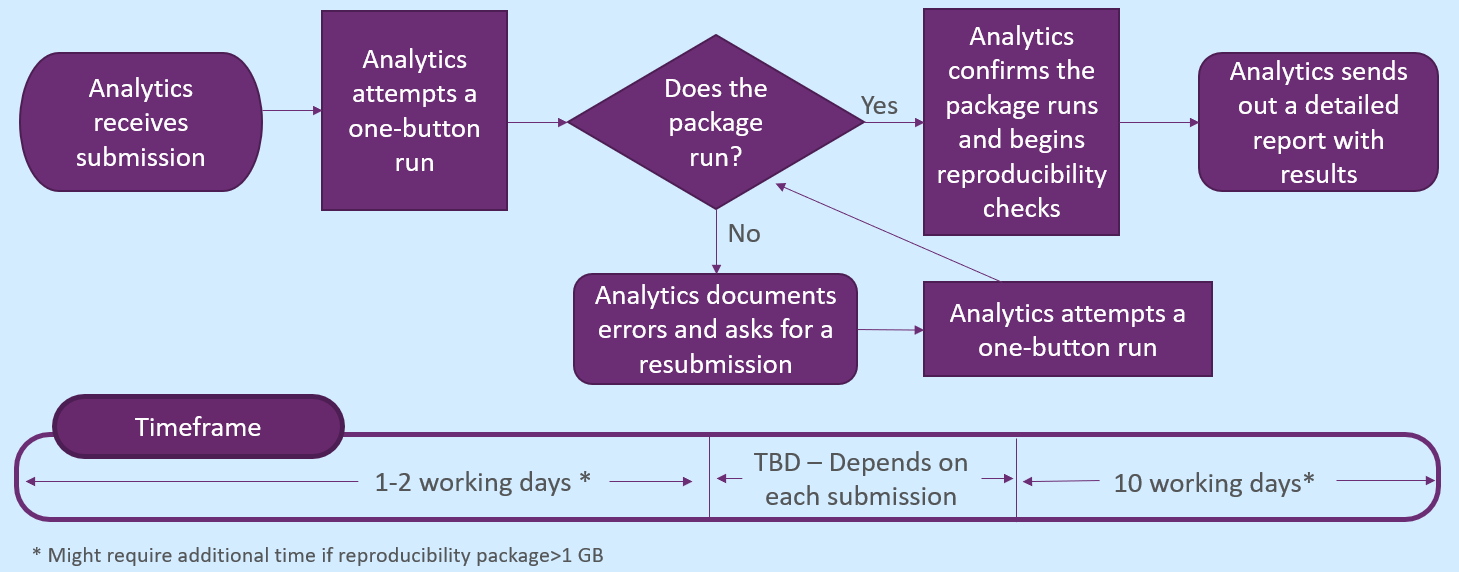
\includegraphics[width=0.9\linewidth]{../img/rep-checks-timeline.png}
	\end{center}

	\bigskip

	After the one-button replication runs, DIME Analytics will check the following:

	\bigskip

	\begin{itemize}
		\setlength\itemsep{-0.1em}
		\item{Regression point estimates and standard errors need to be consistent across the outputs produced by the code and the outputs presented in the academic publication. Marginal differences in point estimates and standard errors might not be problematic, but DIME Analytics will document them shall they occur}
		\item{Any discrepancies observed in the descriptive statistics produced by the output and the statistics mentioned in the academic publication will be documented by DIME Analytics}
		\item{The graphs and visualizations produced by the code will be reviewed as well. This includes checking that the graphs titles, x and y-titles, x and y-ticks, and the graphs legends are consistent across what is produced by the code what is presented in the academic publication}
	\end{itemize}

	\bigskip
	
	This review also entails documenting every specific reproducibility errors (if any), any required installation of packages that are used by the code and suggestions to improve code readability.

	\subsection{3. \, Public release}

	Once this is complete, DIME Analytics can help to organize a public release repository on GitHub (such as \href{https://github.com/worldbank/rio-safe-space}{this example}). Let us know if you would like to do this and we are happy to help you set this up. Many journals now require data and code to be made publicly available, and the World Bank GitHub and Microdata Catalog or Development Data Hub are the recommended resources for this.

	\end{fullwidth}
\end{document}
